
\ifdefined\ishandout
\documentclass[11pt,english,handout]{beamer}
\else
\documentclass[11pt,english]{beamer}
\fi



%\documentclass[11pt]{beamer}
\usepackage{mathptmx}
\renewcommand{\sfdefault}{lmss}
\renewcommand{\familydefault}{\sfdefault}
\usepackage[T1]{fontenc}
\usepackage[latin9]{inputenc}
\usepackage{amsmath}
\usepackage{amssymb}
\usepackage{graphicx}
\PassOptionsToPackage{normalem}{ulem}
\usepackage{ulem}
\usepackage{caption}
\captionsetup{labelformat=empty}
\usepackage{bbm}
\usepackage{upgreek}
\usepackage{graphicx}
\setbeamertemplate{section in toc}[sections numbered]
\makeatletter
\usepackage{caption} 
\captionsetup[table]{skip=10pt}
%%%%%%%%%%%%%%%%%%%%%%%%%%%%%% Textclass specific LaTeX commands.
 % this default might be overridden by plain title style
 \newcommand\makebeamertitle{\frame{\maketitle}}%
 % (ERT) argument for the TOC
 \AtBeginDocument{%
   \let\origtableofcontents=\tableofcontents
   \def\tableofcontents{\@ifnextchar[{\origtableofcontents}{\gobbletableofcontents}}
   \def\gobbletableofcontents#1{\origtableofcontents}
 }


\setbeamersize{text margin left= .8em,text margin right=1em} 
\newenvironment{wideitemize}{\itemize\addtolength{\itemsep}{10pt}}{\enditemize}
\newenvironment{wideitemizeshort}{\itemize}{\enditemize}

%%%%%%%%%%%%%%%%%%%%%%%%%%%%%% User specified LaTeX commands.
%\documentclass[presentation]{beamer}


\def\Tiny{\fontsize{7pt}{8pt}\selectfont}
\def\Normal{\fontsize{8pt}{10pt}\selectfont}

\usetheme{Madrid}
\usecolortheme{lily}
%\setbeamercovered{transparent}
\useinnertheme{rounded}


\setbeamertemplate{footline}{\hfill\Normal{\insertframenumber/\inserttotalframenumber}}
%\setbeamertemplate{footline}{}

\setbeamertemplate{navigation symbols}{}

\newenvironment{changemargin}[2]{%
\begin{list}{}{%
\setlength{\topsep}{0pt}%
\setlength{\leftmargin}{#1}%
\setlength{\rightmargin}{#2}%
\setlength{\listparindent}{\parindent}%
\setlength{\itemindent}{\parindent}%
\setlength{\parsep}{\parskip}% 
}%
\item[]}{\end{list}}

\setbeamertemplate{footline}{\hfill\insertframenumber/\inserttotalframenumber}
\setbeamertemplate{navigation symbols}{}

%\usepackage{times}  % fonts are up to you
\usepackage{graphicx}
%\usepackage{graphics}
\usepackage{epsfig}
\usepackage{bm}
\usepackage{epsf}
\usepackage{float}
\usepackage[final]{pdfpages}
\usepackage{multirow}
\usepackage{colortbl}
\usepackage{xkeyval}
%\usepackage{sgame}
%\usepackage{pst-node}
\usepackage{listings}
\usepackage{ifthen}
%\usepackage{hyperref}
\usepackage{tikz}

%\usepackage{times}  % fonts are up to you
%\usepackage{graphicx}
%\usepackage{graphics}
\usepackage{epsfig,bm,epsf,float}
\usepackage[final]{pdfpages}
\usepackage{xcolor,multirow,colortbl}
\usepackage{xkeyval}
\usepackage{verbatim}
%\usepackage{sgame}
%\usepackage{pst-node}
\usepackage{listings}
%\usepackage{handoutWithNotes}
%\pgfpagesuselayout{3 on 1 with notes}[letterpaper,border shrink=5mm]
%\pgfpagesuselayout{2 on 1 with notes landscape}[letterpaper,border shrink=5mm]
\usepackage{setspace}
\usepackage{ragged2e}

\setbeamersize{text margin left=1em,text margin right=1em} % CambridgeUS spacing if you use default instead


%\pdfmapfile{+sansmathaccent.map}

% Table formatting
\usepackage{booktabs}


% Decimal align
\usepackage{dcolumn}
\newcolumntype{d}[0]{D{.}{.}{5}}

\newcommand\independent{\protect\mathpalette{\protect\independenT}{\perp}}
\def\independenT#1#2{\mathrel{\rlap{$#1#2$}\mkern2mu{#1#2}}}

\global\long\def\expec#1{\mathbb{E}\left[#1\right]}
\global\long\def\var#1{\mathrm{Var}\left[#1\right]}
\global\long\def\cov#1{\mathrm{Cov}\left[#1\right]}
\global\long\def\prob#1{\mathrm{Prob}\left[#1\right]}
\global\long\def\one{\mathbf{1}}
\global\long\def\diag{\operatorname{diag}}
\global\long\def\expe#1#2{\mathbb{E}_{#1}\left[#2\right]}
\DeclareMathOperator*{\plim}{\text{plim}}

%\usefonttheme[onlymath]{serif}

\usepackage{appendixnumberbeamer}
\renewcommand{\thefootnote}{}

\setbeamertemplate{footline}
        {
      \leavevmode%
   %   \hbox{%
%      \begin{beamercolorbox}[wd=\paperwidth,ht=2.25ex,dp=1ex,right]{date in head/foot}%
        %\usebeamerfont{date in head/foot}\insertshortdate{}\hspace*{2em}%
\hfill
    %turning the next line into a comment, erases the frame numbers
        \insertframenumber{}\hspace*{2ex}\vspace{1ex}

  %    \end{beamercolorbox}}%
}

\definecolor{blue}{RGB}{0, 0, 210}
\definecolor{red}{RGB}{170, 0, 0}

\makeatother

\usepackage[english]{babel}

%\mode<handout>{
  %\setbeamercolor{background canvas}{bg=black!5}
  %\usepackage{pgfpages}
  %\pgfpagesuselayout{2 on 1}[a4paper,border shrink=5mm]
 %\pgfpagesuselayout{4 on 1}[a4paper,border shrink=5mm,landscape]
%}
%\newcommand{\opause}{\pause{}} 

\usepackage{tikz}
\newcommand*\circled[1]{\tikz[baseline=(char.base)]{             \node[circle,ball color=structure.fg, shade,   color=white,inner sep=1.2pt] (char) {\tiny #1};}} 

\makeatletter
\let\save@measuring@true\measuring@true
\def\measuring@true{%
  \save@measuring@true
  \def\beamer@sortzero##1{\beamer@ifnextcharospec{\beamer@sortzeroread{##1}}{}}%
  \def\beamer@sortzeroread##1<##2>{}%
  \def\beamer@finalnospec{}%
}
\makeatother

\begin{document}

%% Title slide
\begin{frame}[noframenumbering]{}
\vspace{0.5cm}
\title[]{Chapter 1: Introduction to ECON 1630}
\author{Jonathan Roth}
\date{Mathematical Econometrics I \\ Brown University\\} 
\titlepage {\small{}\ }\thispagestyle{empty} \vspace{-30pt}

\end{frame}
 
\begin{frame}{Outline}

1. Course Preliminaries
\vspace{0.8cm}

2. What is Econometrics?
\vspace{0.8cm}

3. Why is Econometrics Challenging?
\vspace{0.8cm}

4. Course Roadmap

\end{frame}

\begin{frame}{Introducing Ourselves}
\vspace{0.2cm}
Welcome to ECON 1630! I'm looking forward to teaching you all
\vspace{0.5cm}


I'm Professor Jonathan Roth

\begin{itemize}
\item Group OH on Zoom (\href{https://brown.zoom.us/my/jonroth}{\uline{link}}): Mon 220-250 
\item Individual OH: Typically Tue 3-4; sign up on my website: \href{https://jonathandroth.github.io/OfficeHours/}{\uline{here}}, 8 Fones Alley 014 (or Zoom by request)

\end{itemize}
\vspace{0.4cm}

\pause{}

Our Grad TAs are Moritz Poll and Max Grozovsky \\

Our undergrad TAs are Matt Kutam and Preetish Juneja (star students from previous semesters!)

\begin{itemize}
	\item
	All TAs will hold OHs 
	
	\item
	Grad TAs will hold weekly sessions 
	
	\begin{itemize}
		\item 
		Review material and teach coding
	\end{itemize}
	
	\item
	Times/locations for TA OHs  and sections will be announced shortly on Canvas
\end{itemize}
 
\end{frame}

\begin{frame}{Canvas and EdDiscussion}

Course materials and communications will be posted on Canvas: {\url{https://canvas.brown.edu/courses/1100468}} \bigskip 

The Canvas page has an EdDiscussion board, which is a great place to ask (and answer) questions. The TAs will monitor the Qs.

\end{frame}

\begin{frame}
\vspace{0.2cm}
Meeting times:

\begin{itemize}
\item Lectures: Mon/Wed 830-950 (S01) or 3-420pm (S02).\\ \textbf{Recordings will be posted online after class.}
\vspace{0.1cm}
\item TA Sessions: Time/location TBD


\vspace{0.1cm}
\item \textbf{Attendance} is not required but is \textbf{highly encouraged}
\end{itemize}
\vspace{0.3cm}

\pause{}

Prerequisites:

\begin{itemize}
\item Multivariate calculus, probability/statistics, and linear algebra
\vspace{0.1cm}
\item Some familiarity with reading/writing proofs and code
\end{itemize}
\vspace{0.2cm}

\pause{}

Software:

\begin{itemize}
\item Default is Stata for statistical analyses (to be covered in TA sessions)
	\begin{itemize}
		\item 
		You're welcome to use R instead; TAs are familiar with R
	\end{itemize}
\vspace{0.1cm}
\item LaTeX for typing up problem sets (optional, for extra credit)
\vspace{0.1cm}
\item Ask us for help if you're having any problems accessing software
\end{itemize}

\end{frame}

\begin{frame}
\vspace{0.1cm}
Assessments:
\begin{itemize}
\item 6 problem sets due approximately every 2 weeks, submitted via Gradescope
\item 1 midterm exam (November 3, in class)
\item 1 final exam
\vspace{0.1cm}

\end{itemize}
\vspace{0.2cm}

\pause{}

Grading:

\begin{itemize}
\item 30\% problem sets, 35\%  on each exam.
\vspace{0.1cm}
\item
 I'll drop your lowest PSet grade. Use your drop wisely!
\vspace{0.1cm}
\item Psets are due at 4PM on Fridays; late submissions won't be graded.  Collaboration is OK (please list collaborators)
\vspace{0.1cm}
\item The exams will be in-class, closed-book, ``cheat-sheet'' allowed
\vspace{0.1cm}
\item 5 points extra credit if you use LaTeX for assignments. Please attach your code + output as a single PDF regardless
\end{itemize}
\vspace{0.2cm}

\end{frame}

\begin{frame}{AI Policy}

My view is that AI is a useful tool and we shouldn't ignore it. But need to use it in a way that enhances rather than impedes learning. \medskip
	
	\begin{itemize}
		\item \textbf{Exams (70\%):} closed-book; \emph{no AI allowed}.
		\item \textbf{Problem sets:} AI OK if it \emph{helps you learn}, not if it replaces learning/effort.
		\begin{itemize}
			\item \textbf{Good:} debugging R/Stata errors.
			\item \textbf{Bad:} writing free-form answers.
		\end{itemize}
		\item I can't police what you do on the psets, but if you don't put in effort you probably won't do well on the exams
		\item Include brief \textbf{AI use disclosure} on each pset.
	\end{itemize}
	
\end{frame}


\begin{frame}
	Course materials:
	
	\begin{itemize}
		\item Main material: Lectures and lecture slides, which will be posted on Canvas
		
		\item Optional text: Stock \& Watson -- Intro to Econometrics (4th ed)
\end{itemize}
\bigskip
Any questions on logistics? 

\end{frame}

\begin{frame}{Outline}

1. Course Preliminaries $\checkmark$
\vspace{0.8cm}

2. What is Econometrics?
\vspace{0.8cm}

3. Parameters, Estimands, and Estimators
\vspace{0.8cm}

4. Course Roadmap

\end{frame}

\begin{frame}{What is Econometrics?}

\vspace{0.2cm}
$\rightarrow$ The statistical toolkit that economists use to answer economic \uline{questions} with \uline{data}
\bigskip 

What types of questions might we be interested in: 
\pause
\medskip

\begin{itemize}
\item<1-> Has economic inequality increased since 1960?
	\begin{itemize}
		\item<3-> \textbf{Descriptive Q:} asks about how things are (or were) in reality
	\end{itemize}
\item<1-> How do increases in the minimum wage affect employment? 
	\begin{itemize}
		\item<4-> \textbf{Causal Q:} What would have happened in a counterfactual world?  
	\end{itemize}
\item<1->   What will the unemployment rate be next quarter?
	\begin{itemize}
	\item<5-> \textbf{Forecasting Q:} What will happen in the future?  
\end{itemize}

\end{itemize}
\medskip

\pause 
\only<6->{
In this course, we will focus mainly on descriptive and causal questions, with an emphasis on causal questions
}

\end{frame}


\begin{frame}{Why is answering these questions hard?}

\begin{wideitemize}
\item
For descriptive Qs: we only observe data for a \textbf{sample} of individuals, not for the full \textbf{population}
	\begin{itemize}
		\item 
		Example: we want to know how the distribution of income in the US has changed. But we only observe income for a survey of workers
	\end{itemize}
\pause

\item Best case scenario: \\Our sample is \textbf{randomly} selected from the population \\
	\begin{itemize}
		\item 
		E.g., the workers in our survey were drawn out of hat with names of all possible workers
		
		\item
		If so, need to account for the fact that by chance the sample might have different characteristics from the population
	\end{itemize}


\pause
\item Worst case scenario: our sample is \textit{not representative} of the population that we care about
	\begin{itemize}
		\item 
		E.g., workers with certain characteristics were more likely to respond to the survey
	\end{itemize}
\end{wideitemize}

\end{frame}


\begin{frame}
\centering
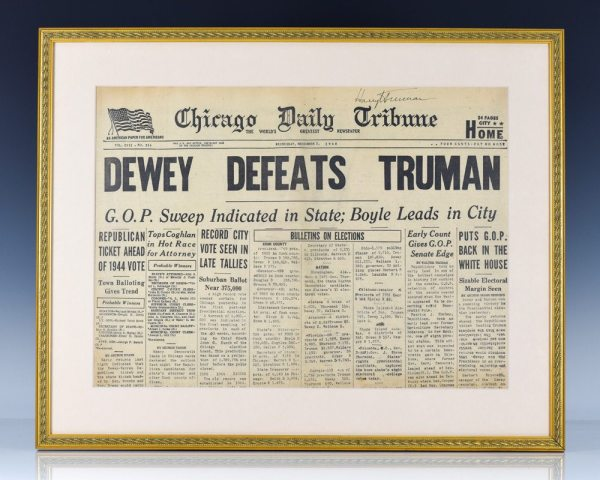
\includegraphics[width = 0.7\linewidth]{dewey-defeats-truman}
\begin{itemize}
	\item 
	In 1948, Chicago Tribune writes that Thomas Dewey defeats Harry Truman in the 1948 presidential election, based on survey of voters.
	
	\pause
	\item
	But their survey was conducted by phone. In 1948, only rich people had phones: sample $\neq$ population $\rightarrow$ misleading results!
\end{itemize}

\end{frame}

\begin{frame}
\textit{Selection bias} referes to settings like Dewey-Truman where the sample is not drawn randomly from the population of interest

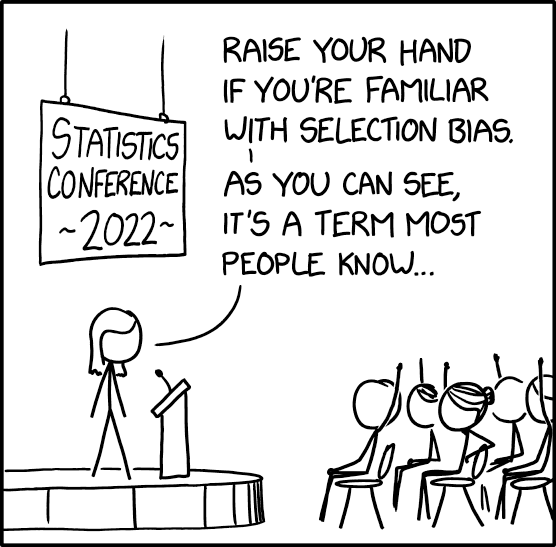
\includegraphics[width = 0.6\linewidth]{selection_bias_xkcd.png}
\end{frame}


\begin{frame}{Why is answering these questions hard? (Part II)}
\begin{wideitemize}
	\item
	Answering causal questions is often \textit{even harder} than descriptive ones. Why?
	
	\pause
	\item
	Causal Qs involve both a descriptive component (what are outcomes in reality?) and a \textit{counterfactual} component (how would things have been under a different treatment?)
	
	\pause
	\item
	Example: what is the causal effect on your earnings of going to Brown instead of URI? 
		\begin{itemize}
			\item
			Descriptive Q: how much do Brown students earn after graduation? 
			
			\item
			Counterfactual Q: how much would Brown students have earned if they went to URI?  
		\end{itemize}
		
	\pause 	
	\item Counterfactual Qs can't ever be answered with data alone. Need additional assumptions to learn about them!	
\end{wideitemize}	
\end{frame}



\begin{frame}{Splitting up the problem}
	\begin{wideitemize}
		
		\item
		When thinking about causal Qs, it's often easier to split the problem in two
		
		\item
		\textbf{Identification:} what could we learn about the parameters we care about (causal effects) if we had the \text{observable data} for the entire population
		\begin{itemize}
			\item 
			Need to make assumptions about how observed outcomes relate to outcomes that would have been realized under different treatments
		\end{itemize}
		
		\item
		\textbf{Statistics}: what can we learn about the full population that we care about from the finite sample that we have?
			\begin{itemize}
				\item 
				Need to understand the process by which our data is generated from the full population
			\end{itemize} 	
		
	\end{wideitemize}	
	
\end{frame}



\begin{frame}{Framework for thinking about these steps}
	
\begin{wideitemize}

\item \textbf{Sample:} the data that you actually observe
	\begin{itemize}
		\item
		A survey of students from Brown and URI graduates about their earnings 
	\end{itemize}

\pause
\item \textbf{Estimator:} a function of the data in the sample 
	\begin{itemize}
		\item Difference in earnings between Brown and URI students in survey
	\end{itemize}

\pause
\item \textbf{Estimand:} a function of the observable data for the \textit{population}
	\begin{itemize}
		\item Difference in earnings between all Brown and URI students 
	\end{itemize}

\pause 
\item \textbf{Target (aka structural) parameter:} what we actually care about
	\begin{itemize}
		\item Causal effect on earnings of going to Brown relative to URI
	\end{itemize}

\end{wideitemize}	

\medskip
\pause
\begin{wideitemize}

\item The process of learning about the \textit{estimand} from the \text{estimator} constructed with your \textit{sample} is called \textbf{statistical estimation/inference}.

\pause 
\item The process of learning about the \textit{parameter} from the \textit{estimand} is called \textbf{identification}.

\end{wideitemize}
	
\end{frame}





\begin{frame}
	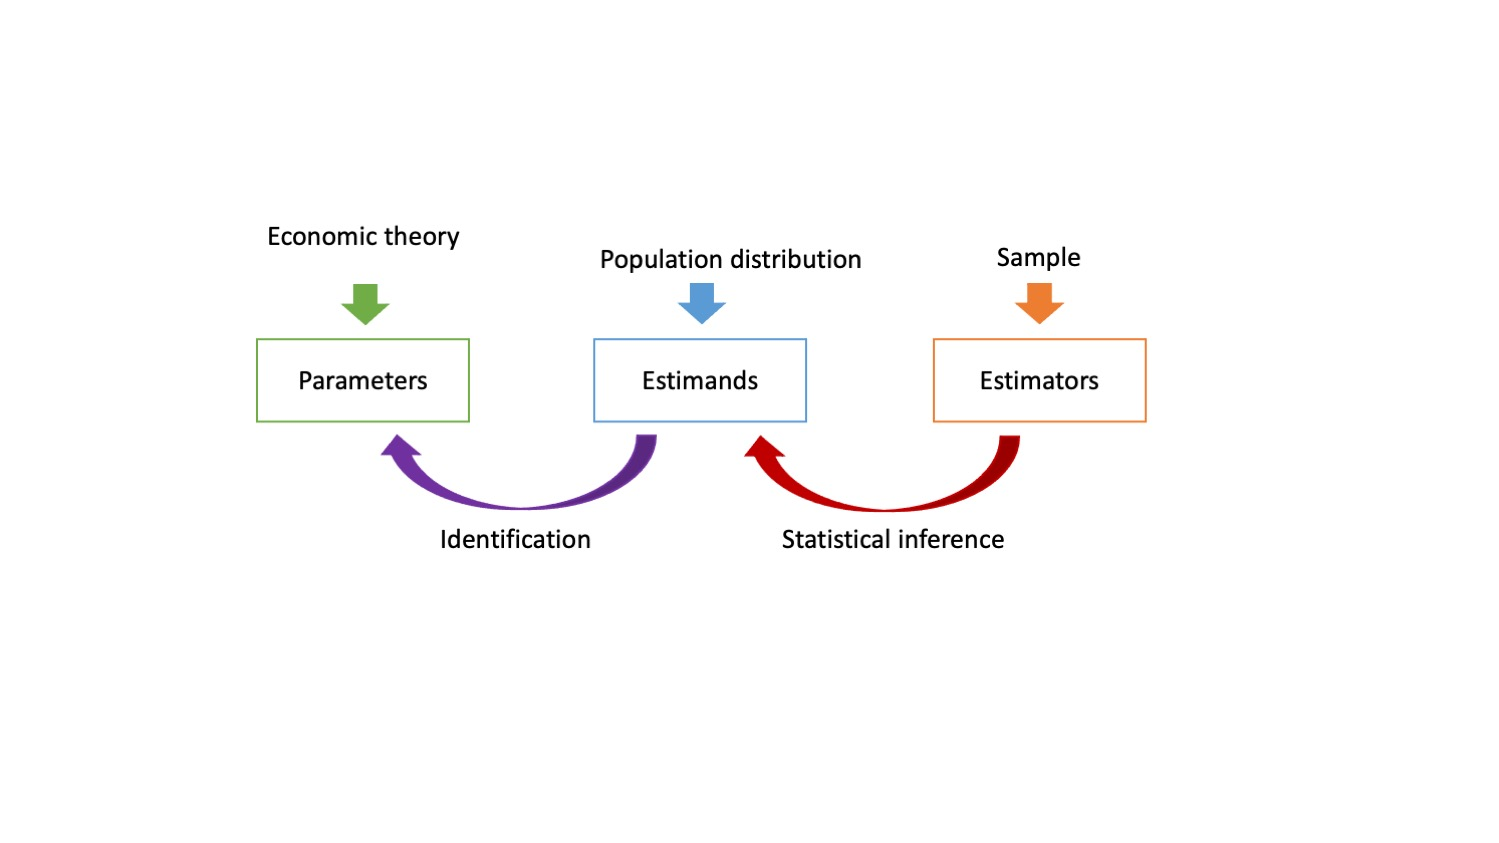
\includegraphics[width=1.2\textwidth]{BigPicture}
\end{frame}


\begin{frame}{Let's add some math...}
\begin{wideitemize}
	\item Introduce \textbf{potential outcomes} notation
		\begin{itemize}
			\item 
			Super useful framework for thinking about causality! \\
			See the 2021 Nobel Prize writeup on Canvas!
		\end{itemize}
	
	\pause 
	\item $D_i$ = indicator if get treatment (1 if Brown, 0 if URI)
	
	\pause
	\item $Y_i(1)$ = outcome under treament = earnings at Brown
	\item $Y_i(0)$ = outcome under control = earnings at URI
	
	\pause 
	\item Observed outcome $Y_i$ is $Y_i(1)$ if $D_i = 1$ and $Y_i(0)$ if $D_i = 0$. ($Y_i$ is your actual earnings)
	
	\pause
	\item
	We can write the observed outcome as $Y_i = D_i Y_i(1) + (1-D_i) Y_i(0)$
\end{wideitemize}

\end{frame}



\begin{frame}
\begin{wideitemizeshort}
	\item
	Example sample: $(Y_i,D_i)$ for $i=1,...N$. Data with earnings and where you went to school
	
	\pause 
	
	\item
	Example estimator: 
		\begin{itemize}
			\item
			Difference in sample mean of earnings for people who went to Brown and people who went to URI: 
			
			$$ \underbrace{\frac{1}{N_1} \sum_{i:D_i=1} Y_i}_{\text{Avg earnings at Brown in sample}} - \underbrace{\frac{1}{N_0} \sum_{i:D_i=0} Y_i}_{\text{Avg earnings at URI in sample}}$$		
		\end{itemize}
	
	\pause
		\item
		Example estimand: 	
		
				\begin{itemize}
			\item
			Difference in population mean of earnings for people went to Brown and people who went to URI: 
			
			$$\underbrace{ E[ Y_i | D_i = 1] }_{\text{Avg earnings at Brown in population}} - \underbrace{E[Y_i | D_i = 0]}_{\text{Avg earnings at URI in population}}$$
		 
		\end{itemize}
	\pause 
	
	\item
	Example target parameter:
		\begin{itemize}
			\item Causal effect of Brown for Brown students:
			$\underbrace{E[Y_i(1) | D_i =1]}_{\text{Earnings at Brown for Brown students in pop}} - \underbrace{E[Y_i(0) | D_i = 1]}_{\text{Earnings at URI for Brown students in pop}} $.   
		\end{itemize}
\end{wideitemizeshort}
\end{frame}


\begin{frame}{Why is causal identification hard?}
	
	\begin{wideitemize}
		
		\item
		Thought experiment: suppose we had data on earnings for \textit{every} Brown and URI graduate
		
		
		\item
		We can learn from the data:
		$$\color{teal} \underbrace{E[ Y_i(1) | D_i=1  ] }_{\text{Earnings at Brown for Brown Students}} \hspace{0.5cm}  \text{and} \hspace{0.5cm} \underbrace{E[Y_i(0) | D_i = 0]	}_{\text{Earnings at URI for URI students}}$$
		
		\pause 
		\item
		The causal effect of Brown for Brown students is 
		$$ \color{teal}{\underbrace{E[ Y_i(1) | D_i=1  ] }_{\text{Earnings at Brown for Brown Students}}} - \color{red}{ \underbrace{E[ Y_i(0) | D_i=1  ] }_{\text{Earnings at URI for Brown Students}}}$$ 
		
		\pause 
		\item
		The data doesn't tell us $\color{red}{ \underbrace{E[ Y_i(0) | D_i=1 ] }_{\text{Earnings at URI for Brown Students}}}$. Why not? 
		\pause
			\begin{itemize}
				\item 
				Because we never see Brown students going to URI!
			\end{itemize} 
		
	\end{wideitemize}
	
\end{frame}


\begin{frame}
	\begin{wideitemize}
		\item
		One idea to solve this problem would be to assume that: 
		
		$$ \color{red}{ \underbrace{E[ Y_i(0) | D_i=1  ] }_{\text{Earnings at URI for Brown Students}}} = \color{teal}{ \underbrace{E[ Y_i(0) | D_i=0 ] }_{\text{Earnings at URI for URI Students}}}$$
		
		\item
		Why might this give us the wrong answer? 
		
		\pause
		
		\item
		Because Brown students may be different from URI students in other ways that would affect their earnings (regardless of where they went to college)
		
			\begin{itemize}
				\item 
				Academic ability, family background, career goals, etc.
			\end{itemize}
		
		\item
		These differences are referred to as \textit{omitted variables} or \textit{confounding factors}
	\end{wideitemize}
\end{frame}

\begin{frame}{What about experiments?}
\begin{wideitemize}
\item
The gold standard for learning about causal effects is a randomized controlled trial (RCT), aka experiment

\item
Suppose that the Brown and URI administration randomized who got into which college (assume these are the only 2 colleges for simplicity)

\item
Since college is randomly assigned, the only thing that differs between Brown and URI students is the college they went to

\item
Hence, 

		$$ \color{red}{ \underbrace{E[ Y_i(0) | D_i=1  ] }_{\text{Earnings at URI for Brown Students}}} = \color{teal}{ \underbrace{E[ Y_i(0) | D_i=0 ] }_{\text{Earnings at URI for URI Students}}}$$
		
		since we've eliminated any confounding factors


\end{wideitemize}
\end{frame}

\begin{frame}{But running experiments is often hard/impossible}
	\begin{wideitemize}
	
	\item
	Unfortunately, Brown/URI have not let us randomize who gets into which college
		\begin{itemize}
			\item
			At least not yet! If you could convince them to do this, it'd make for a cool senior thesis! 
		\end{itemize}


	\item
	Likewise, it is difficult to convince states to randomize their minimum wages, or other policies
	
	\item
	In some cases, randomization is not just difficult but would be immoral 
	
		\begin{itemize}
			\item 
			``What is the causal effect of spousal death on labor supply?''
		\end{itemize}	
	
	\pause
	\item
	In this course, we'll discuss tools economists try to use when running experiments is not possible.
	\end{wideitemize}
\end{frame}

\begin{frame}{Course Roadmap -- Where we're going}
	\begin{wideitemize}
		\item
		\textbf{Part I ($\sim$ 7 lectures): Review of probability/statistics}. This will give us a mathematical language to talk about:
		
			\begin{enumerate}
				\item 
				\textit{Statistical estimation/inference: }how does the sample we observe relate to the population of interest
				
				\item
				\textit{Identification:} how do observable features of the population relate to (causal) parameters we care about
			\end{enumerate}
		\pause 
		
		\item
		\textbf{Part II ($\sim$ 9 lectures): Linear regression: } We'll discuss ordinarly least squares (OLS), the workhorse model for estimation in econometrics. When does it work, and when will it fail?
		
		\pause
		\item
		\textbf{Part III ($\sim$ 7 lectures:) Other ``quasi-experimental'' strategies}: We'll discuss other strategies for ``mimicking'' an experiment when it's not available, including instrumental variables (IV) and regression discontinuity (RD)
			 
	\end{wideitemize}
\end{frame}


\end{document}
}
